\documentclass[12pt,a4paper]{article}
\usepackage[T1]{fontenc}
\usepackage[left=2cm, right=2cm, top=2cm, bottom=2cm]{geometry}
\usepackage{graphicx}
\usepackage{amssymb}
\usepackage{xcolor}
\usepackage{nameref}
\usepackage{enumerate}
\usepackage{placeins}
\usepackage{hyperref}
\title{Formation of Looping Networks - from Nature to Models}
\author{Ali Fele Paranj}

\begin{document}
	\maketitle
	\begin{abstract}
		This is my summary of the international meeting on the ``Formation of Looping Networks - From Nature to Models''.
	\end{abstract}
	
	\section{Introduction: Annemiek Cornelissen, CNRS \& Université de Paris}
	\begin{itemize}
		\item Loops are not stable by design. There should be lots of background mechanisms in action on order to make them stable. [my note: This can also be seen in the papers by Secomb, where he argues that loop is stable only at special conditions].
		\item Mechanisms for the emergence of the loops: 1) Branching along with anastomoses, 2) Structuring from a ``foam''.
	\end{itemize}
	
	\section{The scale of river networks: Olivier Devauchelle, Université de Paris}
	\begin{itemize}
		\item River networks are sparse in loops. However, rivers forming in the deltas are usually  very loopy structures. 
		\item Scallop theorem, first discussed by Purcell in the paper ``Life at low Reynolds number''
	\end{itemize}
	
	
	\begin{figure}[h!]
		\centering
		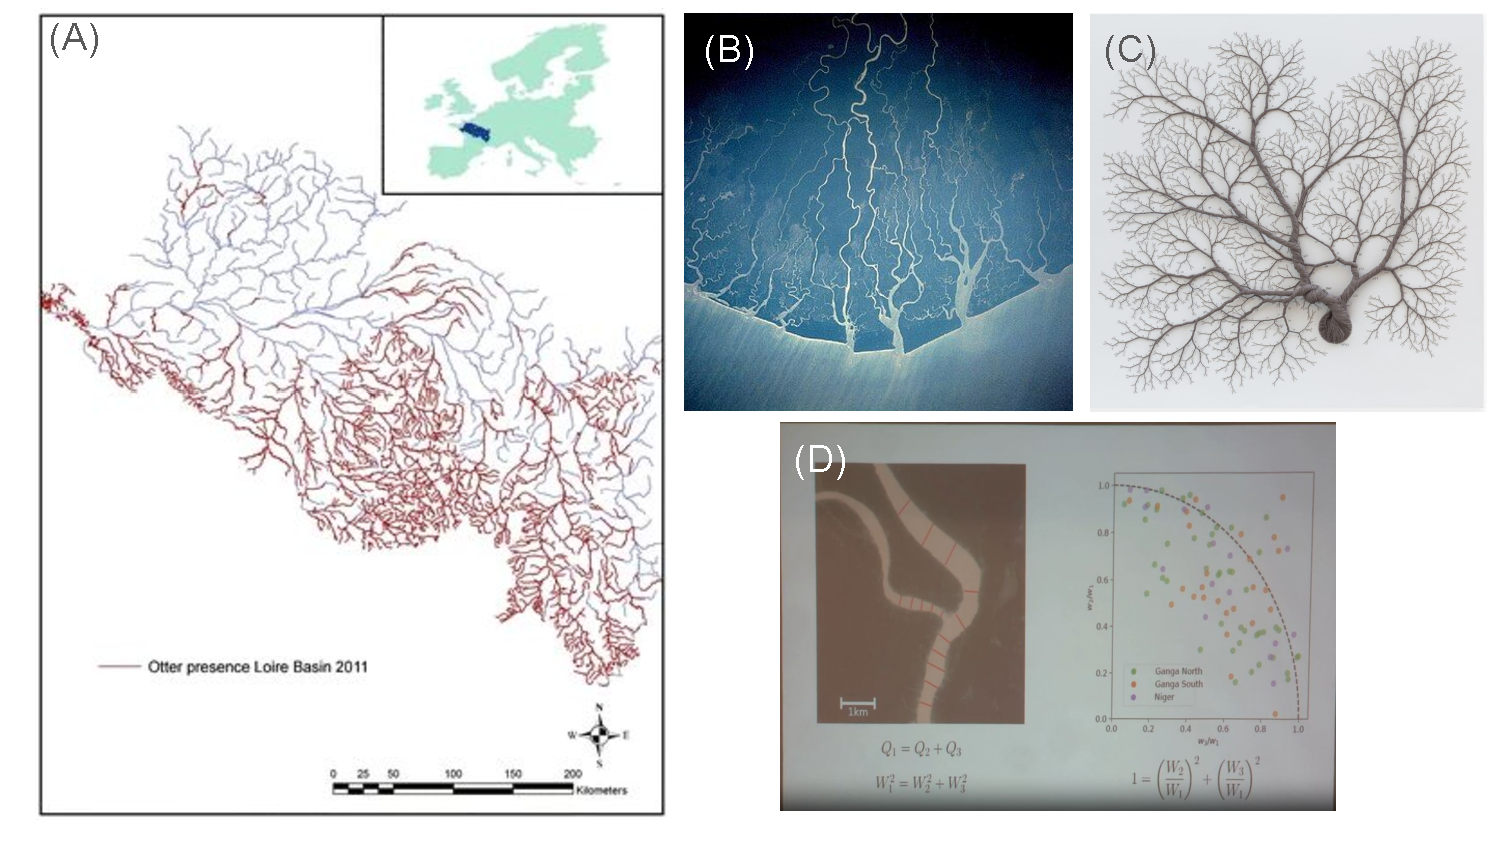
\includegraphics[width=0.7\linewidth]{OlivierTalk.pdf}
		\caption{(A) The basin of the Loire river, France. The low number of loops in the network is noticeable. (B) Niger delta, Nigeria. The are plenty of loops in the river structure. (C) Art piece created by Janaina Mello Landini. (D) A slide of the presentation. Note the relation between the daughter and the parent diameter relation and the real data supporting that relation}
	\end{figure}
	\FloatBarrier
	
	
	\section{River loops morphodynamics: integrating theory with remote sensing observations :Niccolò Ragno, University of Trento}
	\begin{itemize}
		\item Confluence for the rivers is the same as anastomoses for the vascular networks.
		\item Some main questions. 1) Are the loop in the rivers form by pure chance or it is a result of a selective process? 2) Do loops have a characteristic length scale?
	\end{itemize}
	
	\begin{figure}[h!]
		\centering
		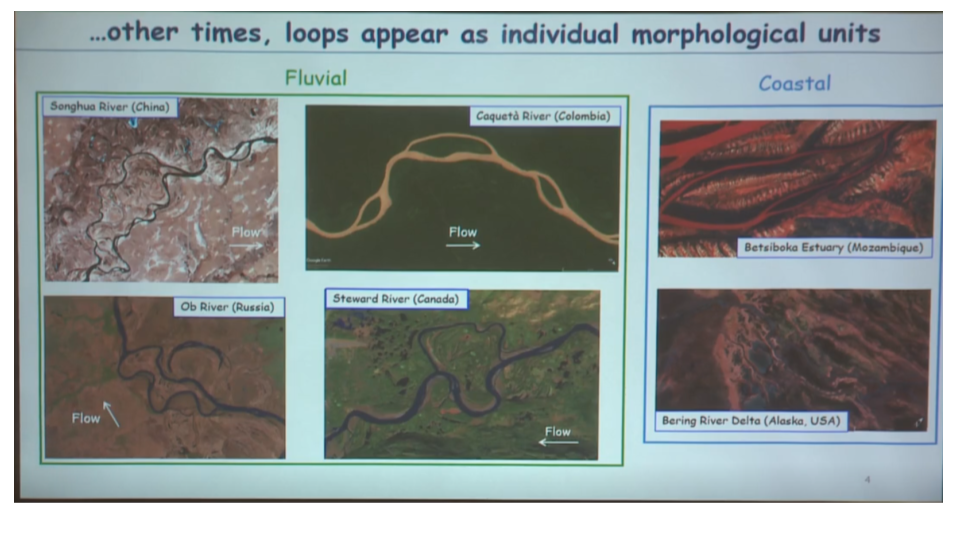
\includegraphics[width=0.7\linewidth]{NiccoloTalk.png}
		\caption{(A) Some beautiful images of loopy networks of rivers. }
	\end{figure}
	
	\FloatBarrier
	
	\section{Tissue geometry and lung branching mode selection: Sharon Lubkin, North Carolina State University}
	\begin{itemize}
		\item A network of networks is a multi-scale network!
	\end{itemize}

	
	\section{From understanding road networks patterns to modeling their evolution: Claire Lagesse, University of Franche-Comté} 
	\begin{itemize}
		\item Take a look at the ``WayMprph'' software.
	\end{itemize}
	
	\begin{figure}[h!]
		\centering
		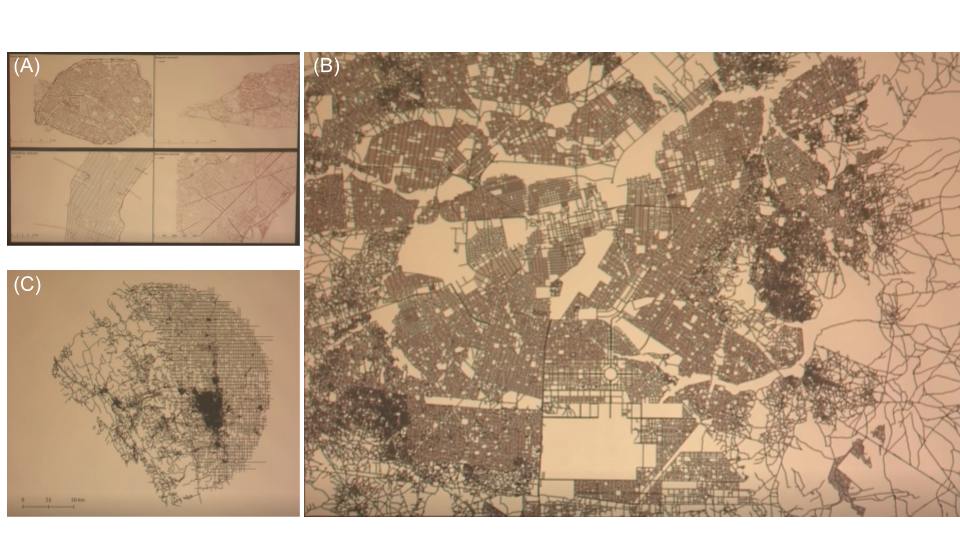
\includegraphics[width=0.7\linewidth]{ClaireTalk.png}
		\caption{(A) Different morphology of cities. (B) Transition of the morphology of the road networks as a function of space. (C) Change of the road network morphology in Calgary. The right part of the graph the road system is more uniform as it is located on a flat ground. However, on the left, the road network is more irregular as it is located in the mountain side of the city.}
	\end{figure}
	
	\FloatBarrier
	
	\section{Developmental Dynamics of Complex, Space-Sharing Networks: To Ensnarl or Not To Ensnarl?Carl Modes, Max Planck Institute of Molecular Cell Biology and Genetics (MPI-CBG)}
	


\end{document}